% Short write-up of ideas for SoLiD neutrino oscillation experiment 
% front-end readout
%
%%%%%%%%%%%%%%%%%%%%%%%%%%%%%%%%%%%%%%%%%
% Arsclassica Article
% LaTeX Template
% Version 1.1 (10/6/14)
%
% This template has been downloaded from:
% http://www.LaTeXTemplates.com
%
% Template author:
% Lorenzo Pantieri (http://www.lorenzopantieri.net) with extensive modifications by:
% Vel (vel@latextemplates.com)
%
% License:
% CC BY-NC-SA 3.0 (http://creativecommons.org/licenses/by-nc-sa/3.0/)
%
%%%%%%%%%%%%%%%%%%%%%%%%%%%%%%%%%%%%%%%%%
\documentclass[
12pt, % Main document font size
a4paper, % Paper type, use 'letterpaper' for US Letter paper
oneside, % One page layout (no page indentation)
%twoside, % Two page layout (page indentation for binding and different headers)
headinclude,footinclude, % Extra spacing for the header and footer
apacite
]{scrartcl}

%%%%%%%%%%%%%%%%%%%%%%%%%%%%%%%%%%%%%%%%%
% Adapted from Arsclassica Article
% Structure Specification File
%
% This file has been downloaded from:
% http://www.LaTeXTemplates.com
%
% Original author:
% Lorenzo Pantieri (http://www.lorenzopantieri.net) with extensive modifications by:
% Vel (vel@latextemplates.com)
% Hacked by David Cussans
% License:
% CC BY-NC-SA 3.0 (http://creativecommons.org/licenses/by-nc-sa/3.0/)
%
%%%%%%%%%%%%%%%%%%%%%%%%%%%%%%%%%%%%%%%%%

%----------------------------------------------------------------------------------------
%	REQUIRED PACKAGES
%----------------------------------------------------------------------------------------

\usepackage{pdfpages}

\usepackage{hyperref}

\usepackage{scrpage2}

\usepackage[T1]{fontenc} % Use 8-bit encoding that has 256 glyphs

\usepackage[utf8]{inputenc} % Required for including letters with accents

\usepackage{graphicx} % Required for including images
\graphicspath{{Figures/}} % Set the default folder for images

\usepackage{enumitem} % Required for manipulating the whitespace between and within lists


\usepackage{subfig} % Required for creating figures with multiple parts (subfigures)

\usepackage{amsmath,amssymb,amsthm} % For including math equations, theorems, symbols, etc

\usepackage{varioref} % More descriptive referencing

\usepackage{tabularx}  % for 'tabularx' environment and 'X' column type
\usepackage{ragged2e}  % for '\RaggedRight' macro (allows hyphenation)
\newcolumntype{Y}{>{\RaggedRight\arraybackslash}X} 
\usepackage{booktabs}
%----------------------------------------------------------------------------------------
%	THEOREM STYLES
%---------------------------------------------------------------------------------------

\theoremstyle{definition} % Define theorem styles here based on the definition style (used for definitions and examples)
\newtheorem{definition}{Definition}

\theoremstyle{plain} % Define theorem styles here based on the plain style (used for theorems, lemmas, propositions)
\newtheorem{theorem}{Theorem}

\theoremstyle{remark} % Define theorem styles here based on the remark style (used for remarks and notes)

%----------------------------------------------------------------------------------------
%	HYPERLINKS
%---------------------------------------------------------------------------------------

\hypersetup{
%draft, % Uncomment to remove all links (useful for printing in black and white)
colorlinks=true, breaklinks=true, bookmarks=true,bookmarksnumbered,
%urlcolor=webbrown, linkcolor=Maroon, citecolor=webgreen, % Link colors
pdftitle={}, % PDF title
pdfauthor={\textcopyright}, % PDF Author
pdfsubject={}, % PDF Subject
pdfkeywords={}, % PDF Keywords
pdfcreator={pdfLaTeX}, % PDF Creator
pdfproducer={LaTeX with hyperref and ClassicThesis} % PDF producer
}
 % Include the structure.tex file which specified the document structure and layout

%----------------------------------------------------------------------------------------
%	TITLE AND AUTHOR(S)
%----------------------------------------------------------------------------------------

\title{SoLi$\delta$ Analogue Front End} % The article title

\author{David Cussans\textsuperscript{1} \& Wim Beaumont\textsuperscript{2}} % The article author(s) - author affiliations need to be specified in the AUTHOR AFFILIATIONS block

\date{} % An optional date to appear under the author(s)

\begin{document}

%----------------------------------------------------------------------------------------
%	HEADERS
%----------------------------------------------------------------------------------------

%% \renewcommand{\sectionmark}[1]{\markright{\spacedlowsmallcaps{#1}}} % The header for all pages (oneside) or for even pages (twoside)
%\renewcommand{\subsectionmark}[1]{\markright{\thesubsection~#1}} % Uncomment when using the twoside option - this modifies the header on odd pages
%\lehead{\mbox{\llap{\small\thepage\kern1em\color{halfgray} \vline}\color{halfgray}\hspace{0.5em}\rightmark\hfil}} % The header style

\pagestyle{scrheadings} % Enable the headers specified in this block

%----------------------------------------------------------------------------------------
%	TABLE OF CONTENTS & LISTS OF FIGURES AND TABLES
%----------------------------------------------------------------------------------------

\maketitle % Print the title/author/date block

\setcounter{tocdepth}{2} % Set the depth of the table of contents to show sections and subsections only

\tableofcontents % Print the table of contents

\listoffigures % Print the list of figures

\listoftables % Print the list of tables
%----------------------------------------------------------------------------------------
%	ABSTRACT
%----------------------------------------------------------------------------------------

\section*{Abstract} % This section will not appear in the table of contents due to the star (\section*)

The design considerations for the front-end readout of the SoLiD neutrino detector are described. The readout chain from the photo-detector to a sampling ADC is described. Circuit simulations are presented, including shaping time, stability and noise.  A SiPMT photo-detector of gain O($10^6$) is assumed, but the circuit could be modified in a straight-forwards manner to accept a single-ended signal from a conventional PMT.


%----------------------------------------------------------------------------------------
%	AUTHOR AFFILIATIONS
%----------------------------------------------------------------------------------------


{\let\thefootnote\relax\footnotetext{\textsuperscript{1} \textit{University of Bristol, United Kingdom}}}

{\let\thefootnote\relax\footnotetext{\textsuperscript{2} \textit{University of Antwerpen, Netherlands}}}

%----------------------------------------------------------------------------------------

\newpage % Start the article content on the second page, remove this if you have a longer abstract that goes onto the second page

\section{Introduction}

The $\mathrm{SoLi}\delta$ neutrino oscillation experiment uses Silicon Photomultipliers ( SiPMT ) coupled to a amplifier/shaper circuit followed by a sampling ADC. The SiPMT has a gain of O($10^6$), similar to a conventional PMT.

SiPMT gain varies rapidly over-voltage ( the amount by which the bias voltage exceeds the break-down voltage). Since the break-down voltage varies between devices it is advantageous to be able to adjust the bias voltage applied to each SiPMT. Since the range of bias voltage adjustment is small O(1V) it is possible to reduce the cost of the bias system by using the SiPMT in a differential circuit using a high voltage bias O(10-100V) common to all SiPMT and individual low voltage trim voltages for each SiPMT. In addition all readily available High accuracy ( > 12 bits ) fast sampling ( > 10MHz ) ADCs use differential inputs. This suggests the use of a fully differential amplifier/shaper circuit (SiPMTs have been used in Particle Physics with differential readout, e.g. \cite{5688208}

\subsection{Circuit Schematic}

Figure~\vref{fig:ada4932_schematic_simplified} shows the circuit schematic for a possible amplifier/shaper together with the SiPMT at the input and the input filter for the ADC at the output.

\begin{figure}[tb]
\centering 
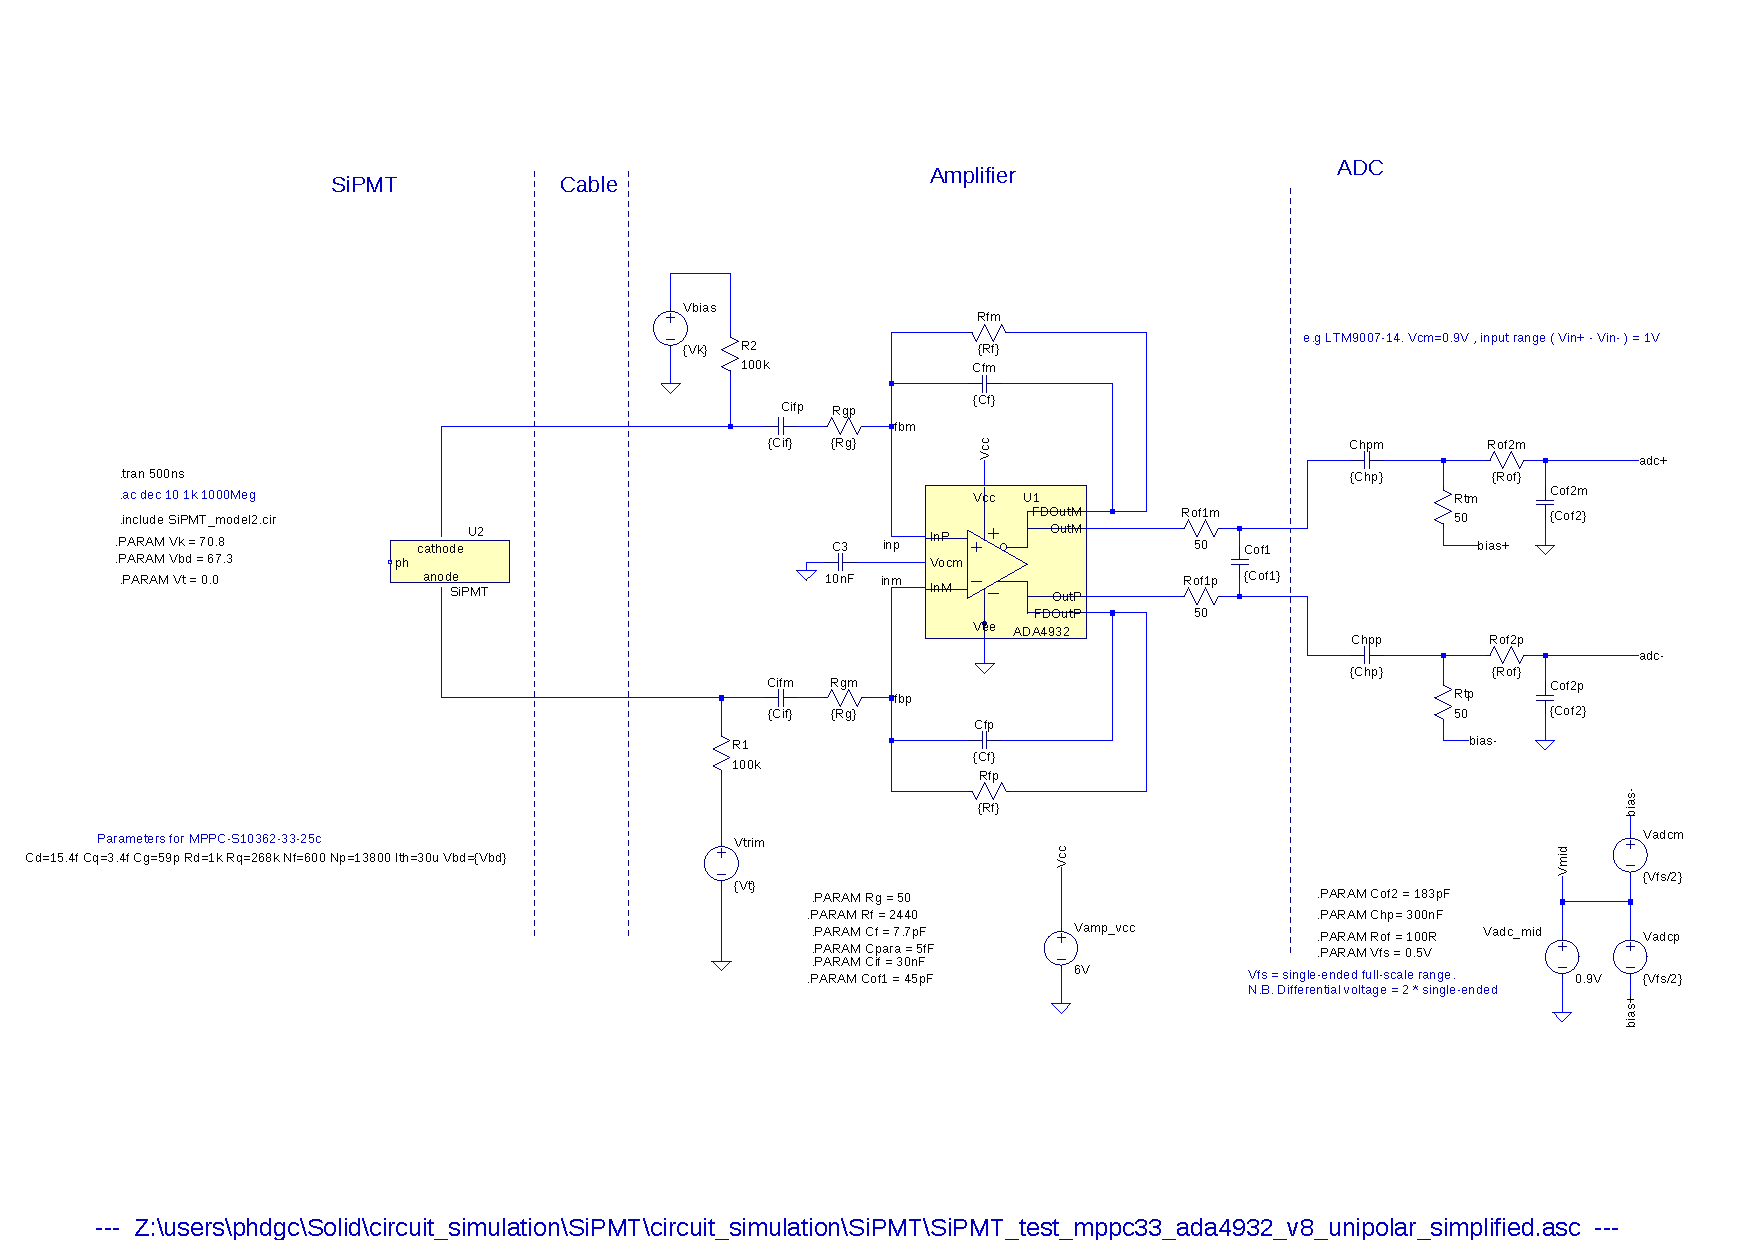
\includegraphics[width=\columnwidth]{SiPMT_test_mppc33_ada4932_v8_unipolar_simplified} 
\caption[Simplified SoLiD amplifier/shaper]{Simplified schematic of an amplifier/shaper circuit for SoLiD. The schematic includes the SiPMT and the filter and biasing components on the ADC+FPGA readout board.} % The text in the square bracket is the caption for the list of figures while the text in the curly brackets is the figure caption
\label{fig:ada4932_schematic_simplified}
\end{figure}


\section{SiPMT Simulation}

In order to predict the affect of the SiPMT capacitance and resistance on the amplifier circuit a detailed simulation of the SiPMT is used. The active macro-cells ( the ones which ``fire'' ) are described by a switched voltage source across a capacitor. The voltage source is disconnected when the current flowing drops below a threshold value, simulating the quenching of the cell. Passive macrocosms are modelled by a resistor and capacitor network. Figure~\vref{fig:active_macrocell} show simplified schematics of the model for the active cells. The model is taken from work described elsewhere \cite{Marano20131}. The parameters in the model need to be matched to the SiPMT being considered. For these simulations parameters matching a Hamamatsu S10362-33-25c~\cite{Hamamatsu_s12572} are used.

For this simulation the SiPMT is run with an over-voltage of 3.5V resulting in a gain of $0.375 \times 10^6$.
\begin{figure}[tb]
\centering 
\subfloat[][Schematic of active cells. The cell firing corresponds to switch $S_0$ closing]{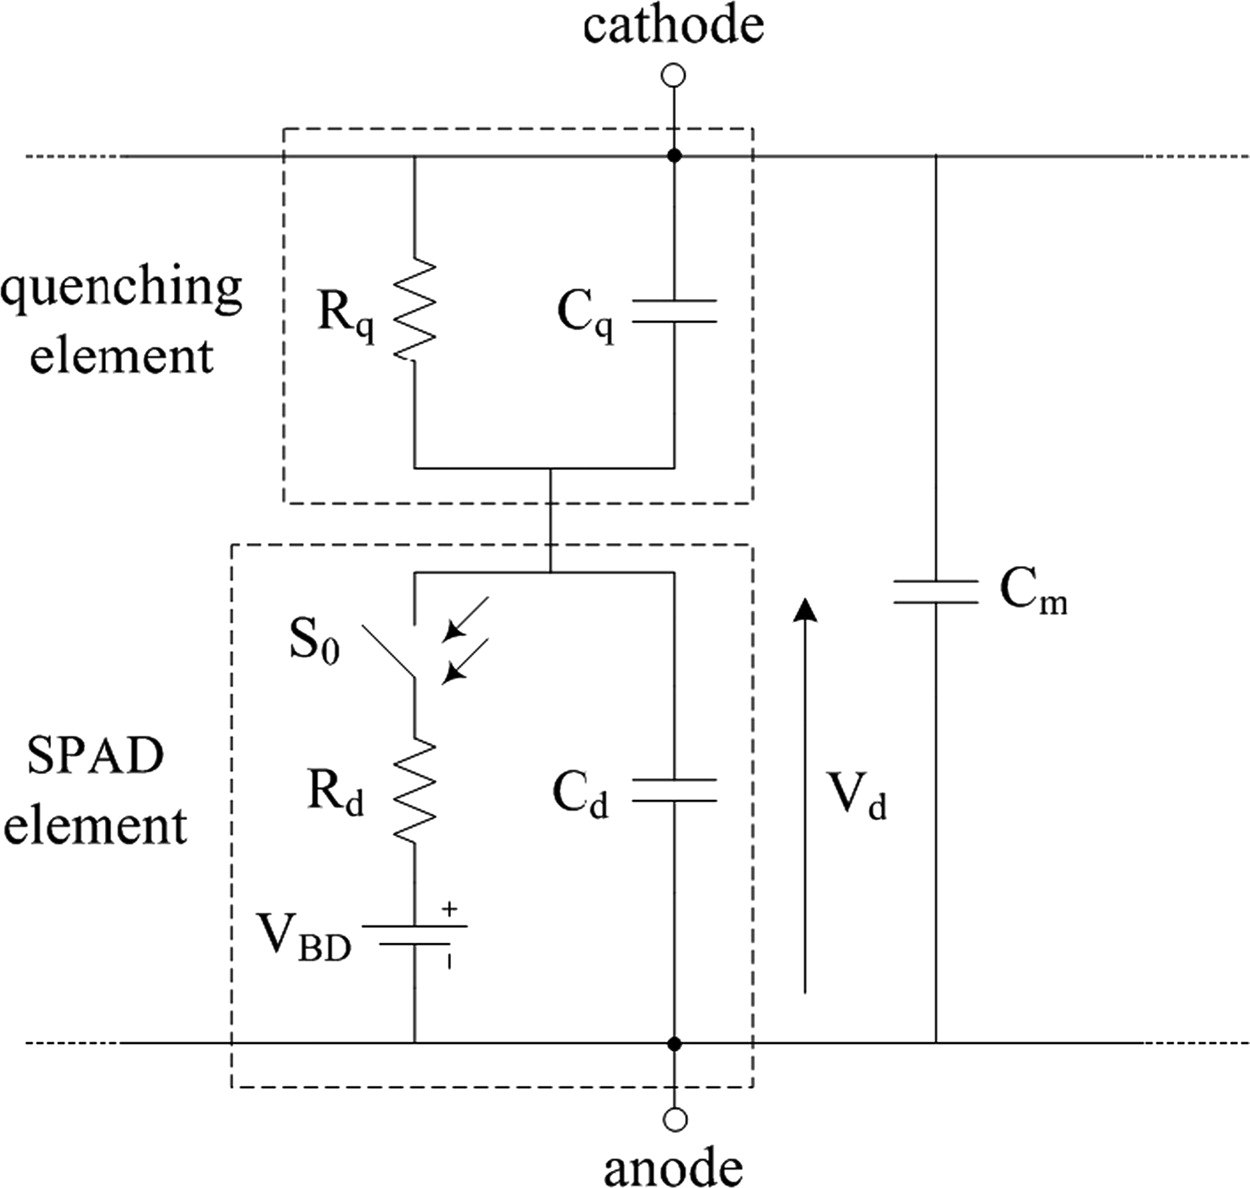
\includegraphics[width=0.5\columnwidth]{simpt_simulation_01.jpg}} 
\subfloat[][Circuit including quenching]{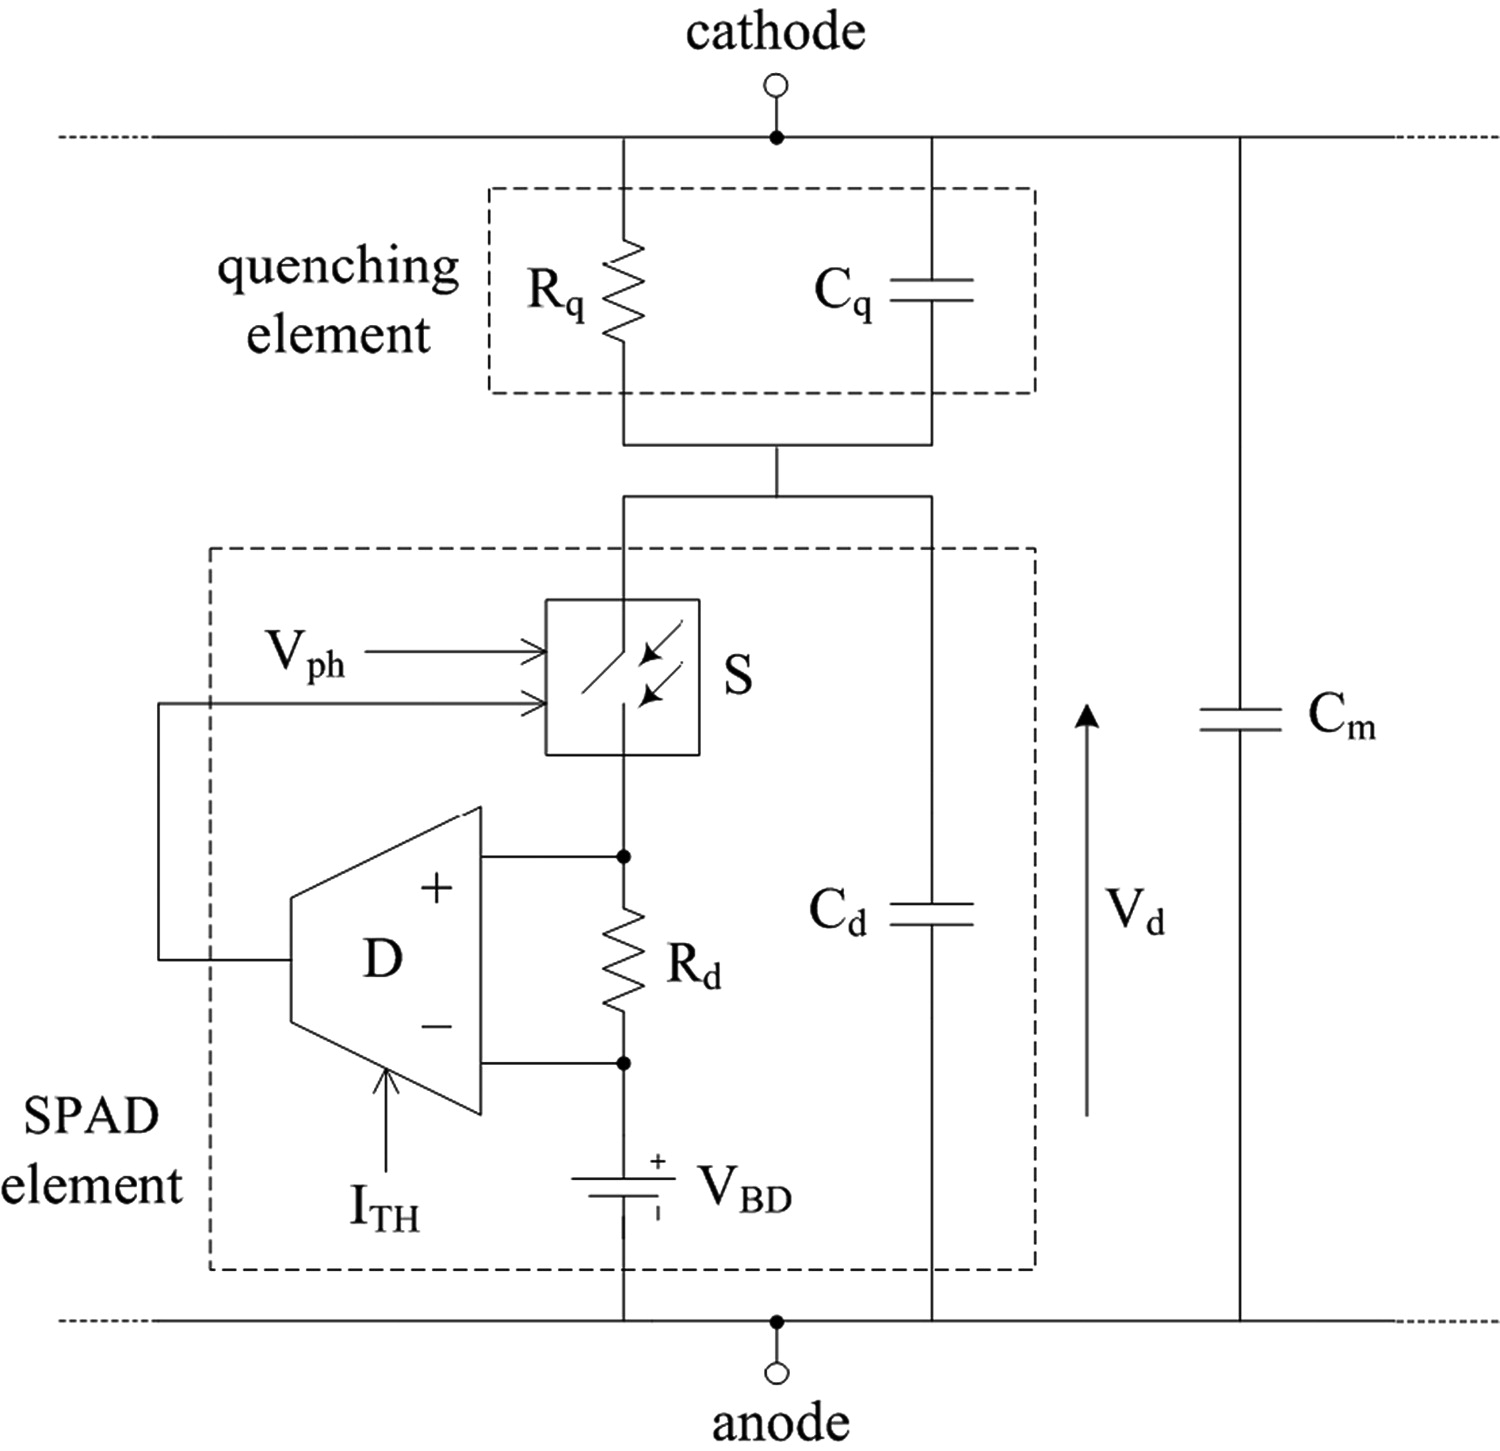
\includegraphics[width=0.5\columnwidth]{simpt_simulation_02.jpg}} 
\caption[SiPMT simulation circuits]{Simplified schematic of a simulation for active cells in SiPMT (a), (b) includes switch for triggering pulse and quenching. An input pulse on $V_{ph}$ closes the switch which then opens when the current drops below $I_{th}$} 
\label{fig:active_macrocell}
\end{figure}


\section{Pulse Shaping}

The amplifier should take the signal from the SiPMT and produce a pulse optimized for sampling by the ADC+FPGA readout board. The amplifier shown in figure~\ref{fig:ada4932_schematic_simplified} has $\mathrm{CR}-(\mathrm{RC})^2-CR-RC$ shaping. The unusual configuration is dictated by the desire to AC couple the input from the SiPMT and the output to the ADC. $(\mathrm{RC})^2$ rather than $(\mathrm{RC})$ shaping was chosen to give a more symmetrical pulse (the fall time is only slightly longer than the rise time. reducing the total pulse width for a given pulse rise time).   

\subsection{Shaping Time}

This implies having enough samples on the rising edge of the pulse to accurately reconstruct pulse height and arrival time. The pulse shaping time should be as short as possible to reduce the amount of ``pile up'' from noise pulses. Optimization of the shaping time should be optimized based on the ADC sample rate, the analogue noise from the amplifier and the rate of ``dark noise'' pulses from the SiPMT. As a starting point an ADC sample rate of $40 \mathrm{MSamples/s}$ was chosen and a peaking time of $60\mathrm{ns}$. This is the sample sample rate/shaping time as chosen by the CMS ECAL\cite{1748-0221-5-03-T03011}.

An simulation of the pulse applied to the ADC inputs by the circuit shown in figure~\vref{fig:ada4932_schematic_simplified} in response to a 600 pixel avalanche pulse is shown in figure~\vref{fig:amplifier_600pa_response}

\begin{figure}[tb]
\centering 
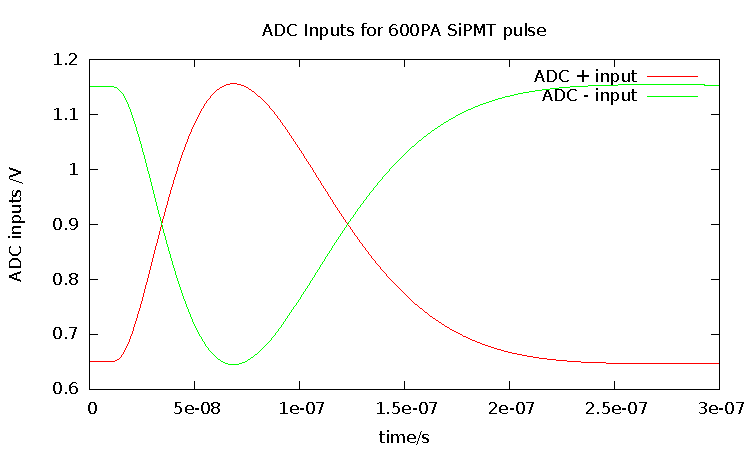
\includegraphics[width=\columnwidth]{SiPMT_test_mppc33_ada4932_v8_unipolar.pdf}
\caption[Simulated signal at ADC input for one 600PA pulse]{Simulated signal at inverting and non-inverting ADC inputs in response to 600PA pulse.}
\label{fig:amplifier_600pa_response}
\end{figure}

\subsection{Unipolar/Bipolar}

Being able to use a low-voltage trim in combination with a single HV bias dictates AC coupling from the SiPMT in some form. Differential ADCs are a mid-scale when the two inputs are at the same voltage. Biasing the ADC so that zero input voltage corresponds to full scale gives one additional bit of dynamic range compared to zero input voltage giving the same voltage at the two ADC inputs. Biasing the ADC inputs in this way implies AC coupling.

If the amplifier is AC coupled a decision has to be made about whether to use unipolar or bipolar shaping. If unipolar shaping is used then if a large number of pulses are received at the input the baseline will drift since the integrated voltage must remain constant over a long time-scale. If bipolar shaping is chosen then the pulse area is zero over a short time-scale.

Bipolar shaping seems initially attractive, since high pulse rates will not result in baseline shift and so the trigger threshold will not need to be adjusted as a function of pulse rate. However in order to trigger on neutrons it is desirable to calculate the total area as well as the maximum amplitude of the pulses. Hence unipolar shaping is almost mandatory for SoLiD.

Figure~\ref{fig:amplifier_600pa_multipulse_response} shows the response of the amplifier to ten 600PA pulses in a period of $2\mu\mathrm{s}$. The baseline shifts by 17mV, corresponding to a shift of 19 pixel-avalanches. The baseline shift reduces to 14mV $2\mu\mathrm{s}$ after the end of the pulses.

\begin{figure}[tb]
\centering 
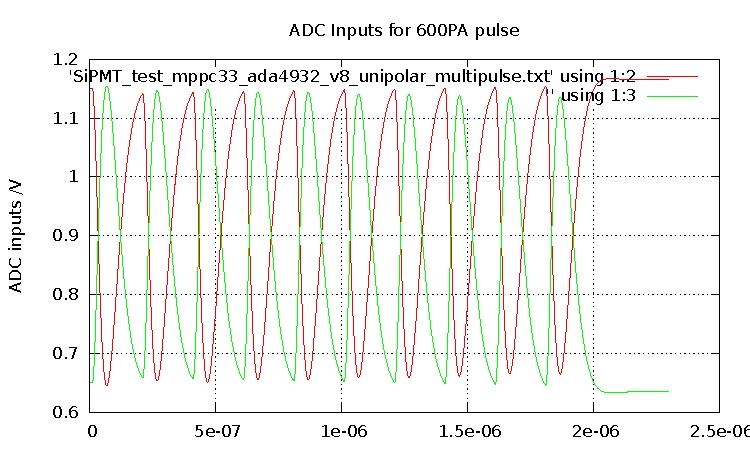
\includegraphics[width=\columnwidth]{SiPMT_test_mppc33_ada4932_v8_unipolar_multipulse.pdf}
\caption[Simulated signal at ADC input for ten 600PA pulses]{Simulated signal at ADC input to ten 600PA pulses over a period of $2\mu\mathrm{s}$. The baseline shifts by an amount equivalent to a pulse height of 19PA.}
\label{fig:amplifier_600pa_multipulse_response}
\end{figure}

\subsection{Component Values}

Table~\vref{tab:component_values} lists the component values in the simulated circuit. A neutron light output time of $10\mu\mathrm{s}$ is assumed.

\begin{table}[tb]
\centering
\begin{tabularx}{\textwidth}{|l|l|X|} % Columntype Y declared in structure.tex
%\begin{tabular}{|l|l|l|} % Columntype Y declared in structure.tex
 Components & Value &  Comments \\
\toprule % from booktabs

$\mathrm{C}_\mathrm{ifp}$ , $\mathrm{C}_\mathrm{ifm}$ & $30\mathrm{nF}$ & Together with $\mathrm{R}_\mathrm{g}$ and the output impedance of the SiPMT forms a high-pass filter that blocks the DC bias to the SiPMT.  The RC time-constant should be larger than the neutron light output time.\\ \midrule

$\mathrm{R}_\mathrm{gp}$ , $\mathrm{R}_\mathrm{gm}$ & $50\Omega$ & Together with $\mathrm{C}_\mathrm{if}$ and the output impedance of the SiPMT forms a high-pass filter. Together with $\mathrm{R}_\mathrm{f}$ and  $\mathrm{C}_\mathrm{f}$ sets the gain of the amplifier. Sets the input impedance at medium frequency, so should be set to half the cable characteristic impedance.\\ \midrule

$\mathrm{C}_\mathrm{fp}$ , $\mathrm{C}_\mathrm{fm}$ &  $7.7\mathrm{nF}$ & Together with $\mathrm{R}_\mathrm{f}$ sets the gain and shaping time of the amplifier  \\ \midrule

$\mathrm{R}_\mathrm{fp}$ , $\mathrm{R}_\mathrm{fm}$ &  $2440\Omega$ & Together with $\mathrm{C}_\mathrm{f}$ sets the gain and shaping time of the amplifier  \\ \midrule

$\mathrm{R}_\mathrm{of1m}$ , $\mathrm{R}_\mathrm{of1p}$ &  $50\Omega$ & Together with $\mathrm{C}_\mathrm{of1}$ forms a RC low pass filter. Set $\mathrm{R}_\mathrm{of1}\mathrm{C}_\mathrm{of1}/2 = \mathrm{R}_\mathrm{f}\mathrm{C}_\mathrm{f}$. Also sets the output impedance at low frequency \\ \midrule

$\mathrm{C}_\mathrm{of1}$  &  $45\mathrm{pF}$ &  \\ \midrule

$\mathrm{C}_\mathrm{hpp}$ , $\mathrm{C}_\mathrm{hpm}$ &  $300\mathrm{nF}$ & Together with $\mathrm{R}_\mathrm{t}$ forms a high-pass filter that allows the DC bias to the ADC to be set. The RC time-constant should be larger than the neutron light output time. \\ \midrule

$\mathrm{R}_\mathrm{tp}$ , $\mathrm{R}_\mathrm{tm}$ &  $50\Omega$ & Sets the input impedance of the ADC at high frequency. \\ \midrule

$\mathrm{R}_\mathrm{of2m}$ , $\mathrm{R}_\mathrm{of2p}$ &  $100\Omega$ & Together with $\mathrm{C}_\mathrm{of2}$ forms a RC low pass filter. Set $\mathrm{R}_\mathrm{of2}\mathrm{C}_\mathrm{of2} = \mathrm{R}_\mathrm{f}\mathrm{C}_\mathrm{f}$. \\ \midrule

$\mathrm{C}_\mathrm{of2p}$ , $\mathrm{C}_\mathrm{of2m}$ &  $183\mathrm{pF}$ &  \\
\bottomrule

%\end{tabular}
\end{tabularx}
\caption{Component values for amplifier/shaper}
\label{tab:component_values}
\end{table}

\section{Cross-Talk between Channels}

Signals in one channel will induce signals in adjacent channels. The amount of cross talk is difficult to simulate but experience suggests it will probably be in the range 1 - 2 \% . Reducing cross talk is possible, but would require more time to perform PCB layout, increased number of interactions and more expensive connectors. This should be justified by simulation of the physics requirements.

\section{Input/Output Impedance}

In order to preserve maximum flexibility for location of the amplifier/shaper ( close to the SiPMT / close to the ADC / cables to both ) the input and output impedance should be matched to the characteristic impedance of a differential cable ( typically $100\Omega$ ). 
 
\section{Noise Requirements}

The dynamic range for the amplifier is set by wanting to be able to measure signals as small as one pixel avalanche ( in order to calibrate the SiPMT gain ) and as large as five times the most probable energy deposit from a cosmic ray muon in order to calibrate the light output from the cubes. In SM1, five times the most probable energy deposit from a cosmic ray muon corresponds to approximately 600 PA~\cite{ref:cosmic_calibration}

Full scale differential voltage range of the ADC is $1-2\mathrm{V}$ ( i.e. the voltage swing of each input is $0.5-1\mathrm{V}$). If a differential voltage range of 1V and a full scale of 600PA is assumed this corresponds to differential voltage of $1.7\mathrm{mV}/\mathrm{PA}$, or voltage of $850\mu\mathrm{V}/\mathrm{PA}$ at each ADC input for each pixel avalanche. If it is desired to have 10 ADC counts per PA this implies $85\mu\mathrm{V}/\mathrm{count}$. Ideally the RMS noise should be less than one ADC count.

\subsection{Noise Simulation}

Figure~\vref{fig:noise_simulation} shows the simulated output
noise. The thermal noise of the resistors and most of the noise
sources inside the Op-amp are simulated. Integrated between 100Hz and
1GHz the simulation predicts an RMS noise at each ADC input of
$28\mu\mathrm{V}$ , comfortably below the target of
$85\mu\mathrm{V}$. In fact the effect of this noise would be even lower, since several samples would be summed to estimate the charge in a pulse. However, it should be emphasized that the
simulation only includes internally generated noise from the amplifier
circuit, it does not include the effect of external noise picked up on
cables etc.

\begin{figure}[tb]
\centering 
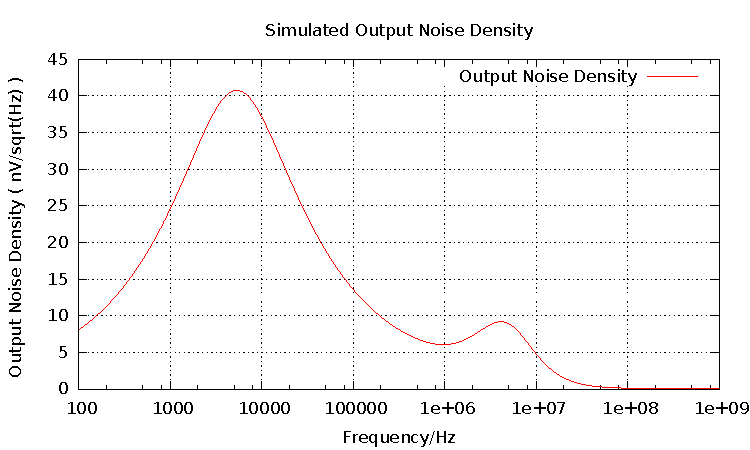
\includegraphics[width=\columnwidth]{SiPMT_test_mppc33_ada4932_v8_unipolar_noise.pdf}
\caption[Simulated output noise at  ADC input]{Simulated noise at  ADC input. Thermal noise from resistors and most sources of noise inside the op-amp are included.}
\label{fig:noise_simulation}
\end{figure}


\section{Amplifier Choice/Stability Considerations}

The amplifier/shaper needs to be stable at all frequencies. One way of verifying this in simulation is to simulate the open loop gain. In an ideal inverting amplifier circuit, if the feedback loop between the amplifier output and input is broken and a voltage applied to the inputs an infinite signal is generated at the circuit node that was connected to the input before the loop was opened. This signal is $180^\circ$ out of phase with the input signal. Hence, when the loop is closed this feedback ensures that the input is always a ``ground''. A real ( non-ideal ) amplifier has finite gain and a non-zero phase-shift, both of which vary with frequency. If the feedback components, or the amplifier, are badly chosen the open-loop phase shift can drop to $0^\circ$ at a frequency where the gain is > 1 and the circuit will oscillate. A ``rule of thumb'' is that the phase shift should not drop below $45^\circ$ at any frequency where the amplifier gain is greater than unity (i.e.. the phase margin should be greater than $45^\circ$ ).

The operational amplifier should be chosen so that the bandwidth is high enough that the pulse shape depends almost entirely on the passive components in the feedback network but should also have gain/phase characteristics that ensure the amplifier is stable.

Figure~\vref{fig:phase_margin} shows the open-loop gain for the circuit shown in figure~\ref{fig:ada4932_schematic_simplified} with two different amplifiers, the Analogue Devices ADA4932 and the Linear Technologies LTC6404-4. The bandwidth of the ADA4932 is only just sufficent for the circuit but it gives a phase margin of $48^\circ$. The LTC6404-4 has a higher bandwidth but gives a phase margin of  $24^\circ$ which is likely to result in an amplifier/shaper that oscillates or ``rings'' in response to pulses.

\begin{figure}[tb]
\centering 
\subfloat[][Open Loop Gain with LTC6404-4]{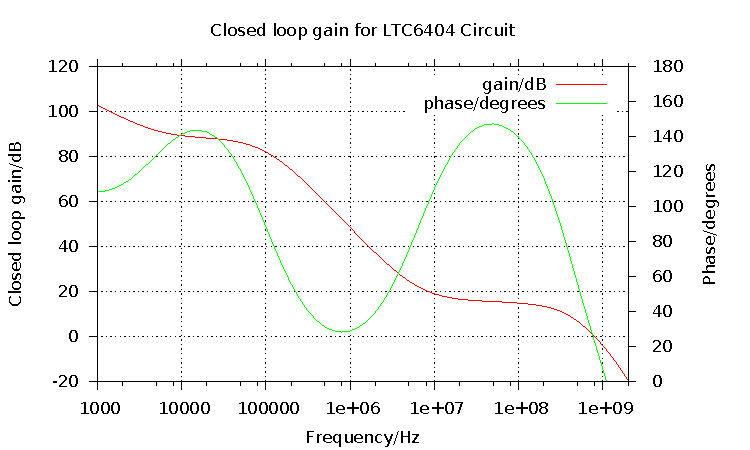
\includegraphics[width=0.5\columnwidth]{SiPMT_test_mppc33_ltc6404_closed_loop_v8a.pdf}} 
\subfloat[][Open Loop Gain with ADC4932]{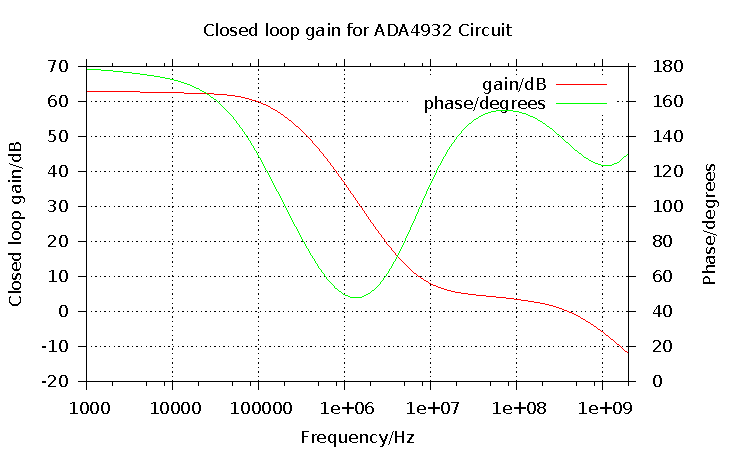
\includegraphics[width=0.5\columnwidth]{SiPMT_test_mppc33_ada4932_closed_loop_v8.pdf}} 
\caption[Closed loop gain with different Op-amps]{Open loop gain for amplifier shaper for (a) LTC6404-4 with a phase margin of $24^\circ$ and (b) ADA4932 with a phase margin of $48^\circ$} 
\label{fig:phase_margin}
\end{figure}

%\renewcommand{\refname}{\spacedlowsmallcaps{References}} % For modifying the bibliography heading

\bibliographystyle{unsrturl}

\bibliography{solid_sipmt.bib} % The file containing the bibliography

%----------------------------------------------------------------------------------------

\end{document}
